\documentclass[10pt,a4paper]{article}
\usepackage[utf8]{inputenc}
\usepackage{tikz}
\usetikzlibrary{calc}
\begin{document}
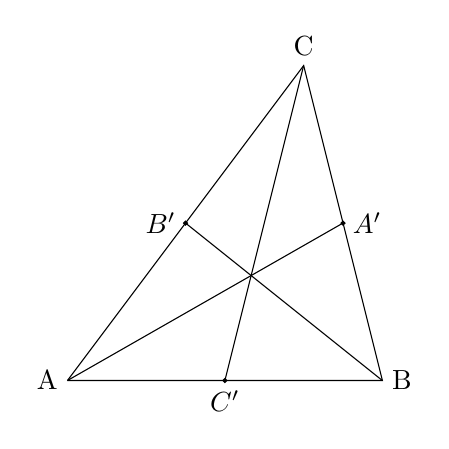
\begin{tikzpicture}[x={10.0mm},y={10.0mm}]
\coordinate (A) at (0,0);
\coordinate (B) at (4,0);
\coordinate (C) at (3,4);
\draw (A) -- (B) -- (C) -- (A);
\node [left] at (A) {A};
\node [right] at (B) {B};
\node [above] at (C) {C};

\coordinate (Aprime) at ($(B)!0.5!(C)$);
\draw[fill] (Aprime) circle [radius = 0.025];
\node [right] at (Aprime) {$A'$};

\coordinate (Bprime) at ($(A)!0.5!(C)$);
\draw[fill] (Bprime) circle [radius = 0.025];
\node [left] at (Bprime) {$B'$};

\coordinate (Cprime) at ($(B)!0.5!(A)$);
\draw[fill] (Cprime) circle [radius = 0.025];
\node [below] at (Cprime) {$C'$};

\draw (A) -- (Aprime);
\draw (B) -- (Bprime);
\draw (C) -- (Cprime);

\end{tikzpicture}
\qquad 
\begin{tikzpicture}[x={10.0mm},y={10.0mm}]
\coordinate [label = left: $A$](A) at (3,3);
\coordinate [label = right: $B$](B) at (5,4);

\draw (A) -- (B);

\draw (A) let \p1 = ($(B) -(A)$) in circle ({veclen(\x1,\y1)});


\end{tikzpicture}
\end{document}